\chapter{Mobile Manipulators Control Problem}
\label{chapter4}
We have previously seen that Mobile Manipulators are systems where locomotion and manipulation tasks are held simultaneously. The coordination of this two tasks is not trivial since the mobile platform combined with the manipulator is a redundant system, so the same point in workspace can be reached moving the mobile base, or moving the manipulator, or with a combined motion of the two. In addition to this kinematic issue, also the dynamic interaction between mobile base and manipulator should be taken into account in a control logic. \\
In literature the control of mobile manipulators mainly followed two strategies. The first approach is the separate control of the mobile base and of the manipulator arm, considering later their interaction. With this approach is possible to simply solve the kinematic redundancy of the system. A reference for this approach can be \cite{liulewis} or \cite{chung1998interaction}. The second approach is the coordination of the motion of both the base and the manipulator through the control of the whole integrated redundant system choosing one configuration among the infinite possible ones with a suitable criterion.\\
We will split this chapter in the description of the control of the mobile base, followed in the second section by the problem of the integration of the manipulator in the control.
\section{Control of Mobile Robots}
Facing the control of a mobile platform it is needed to deal with a nonholonomic system, which is nonlinear.
Usually for the control of the mobile base motion the kinematic model is used applying as inputs to the system the commands for the longitudinal velocity $v$ and the steering velocity $\omega$. In this way it is possible to control directly the generalized velocities of the base, i.e. $\dot{x}_b,\dot{y}_b,\dot{\theta}_b$, through the nonholonomic relation \ref{G}.
It would be certainly possible to use a dynamic based control of the motion giving torques commands to the wheels of the base, but in most mobile robots, in particular in the one we have used, the dynamic perturbation is very small, or it could be canceled through a proper state feedback. Moreover a common charachteristics of commercially available mobile platforms is that it is possible to give the mobile robot only velocity commands.\\
The control of the mobile base can be implemented in two ways: regulation, i.e. driving the robot to a constant position and/or orientation, and trajectory tracking, i.e. forcing the robot to follow a time-varying reference trajectory.
\subsection{Regulation}
The regulation problem can be addressed in two ways.
\subsubsection{Cartesian Regulation}
\begin{figure}[h!]
	\centering
	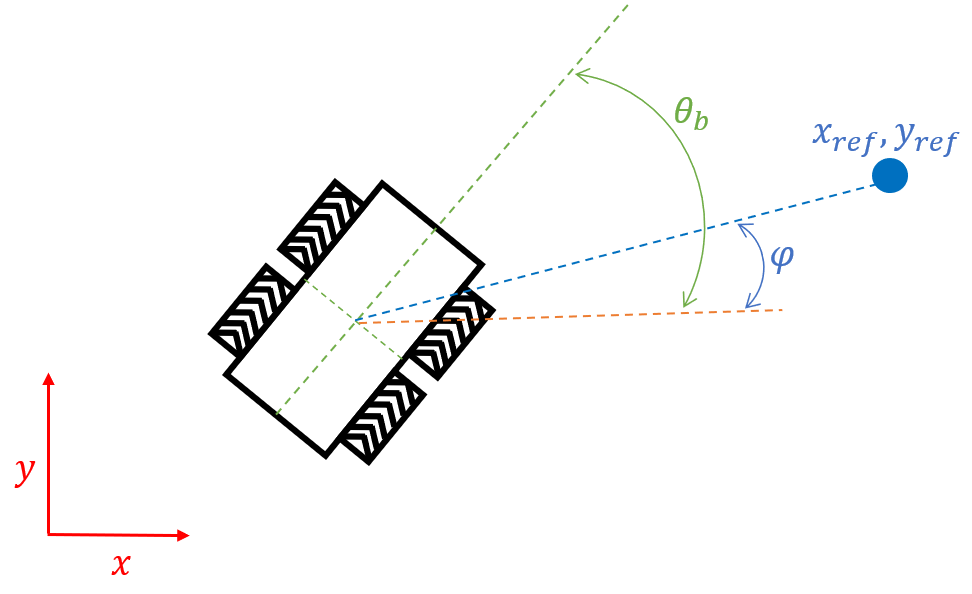
\includegraphics[scale=0.7]{cartesian_regulation}
	\caption{Cartesian Regulation problem}
	\label{cartregulation} 
\end{figure}
The robot (a unicycle) has to reach a point whose coordinates $(x_{ref},y_{ref})$ are defined in the Cartesian space. In this problem there is no need to control also the orientation of the robot. 
In literature several control laws have been proposed. Among others \cite{siciliano} reports: defining the Cartesian error $$\mathbf{e}_P=(x_{ref}-x_b,y_{ref}-y_b)=(e_{P_x},e_{P_y})$$ the control inputs can be obtained as
\begin{align}
	v &= k_1(e_{P_x}\cos\theta_b+e_{P_y}\sin\theta_b)\\
	\omega &= k_2\left(\text{Atan2}\left(e_{P_y},e_{P_x}\right)-\theta_b-\pi\right)
\end{align}
where $k_1$ and $k_2$ are positive constants. 
As \cite{siciliano} too says, these commands can be directly interpreted seeing $v$ has the an input proportional to the Cartesian error, driving the robot to $\mathbf{e}_P=0$, while $\omega$ is steering the robot in the direction pointing to $(x_{ref},y_{ref})$, i.e. $\omega$ is proportional to the difference $\theta-\varphi$, where $\varphi$ is $\text{Atan2}\left(e_{P_y},e_{P_x}\right)$ as can be seen in Figure \ref{cartregulation}.
\subsubsection{Posture Regulation}
The robot has to get to a certain configuration, i.e. Cartesian position and orientation. 
Also in this case, the literature is full of control laws for this kind of problem. We report the control law found in \cite{dixon} and in \cite{samson}.
Defining, for a practical advantage, the transformation:
\begin{equation} \label{trackingerrortransformation}
 	\mathbf{e}=
 	\left[\begin{matrix}
		e_1\\e_2\\e_3
	\end{matrix}\right] = 
	\left[\begin{matrix}
		\cos\theta_b & \sin\theta_b & 0 \\
		-\sin\theta_b & \cos\theta_b & 0 \\
		0 & 0 & 1
	\end{matrix}\right]
	\left[\begin{matrix}
	x_{ref}-x_b\\y_{ref}-y_b\\\theta_{ref}-\theta_b
	\end{matrix}\right]
\end{equation}
where $\mathbf{e}$ is the vector of the errors in the local frame of the mobile robot. In particular $e_1$ is the error in the longitudinal direction and $e_2$ is the error in the transversal direction.\\ Deriving the above equation taking into account the kinematic relation \ref{G}:
\begin{equation}
	\left[\begin{matrix}
		\dot{e}_1\\\dot{e}_2\\\dot{e}_3
	\end{matrix}\right] = 
	\left[\begin{matrix}
		-v+\omega e_2\\-\omega e_1\\\omega
	\end{matrix}\right]
\end{equation}
The proposed control law for $v$ and $\omega$ is:
\begin{equation}
	\left[\begin{matrix}
	v\\\omega
	\end{matrix}\right] = 
	\left[\begin{matrix}
	-k_1e_1\\-k_2e_3+e_2^2\sin(t)
	\end{matrix}\right]
\end{equation}
where $k_1$ and $k_2$ are positive constants. So the closed-loop dynamics becomes:
\begin{equation}
	\left[\begin{matrix}
	\dot{e}_1\\\dot{e}_2\\\dot{e}_3
	\end{matrix}\right] = 
	\left[\begin{matrix}
	k_1e_1+\omega e_2\\-\omega e_1\\-k_2e_3+e_2^2\sin(t)
	\end{matrix}\right]
\end{equation}
Note that the closed-loop dynamics for $e_3$ is a linear system subjected to a nonlinear additive disturbance. Anyway it remains stable as long as this disturbance remains bounded. For the stability proof of this control law we refer to \cite{dixon}.
\subsection{Trajectory Tracking}
Controlling that the robot follows a certain trajectory not only means to make it track a path, i.e. the locus of points which the robot has to follow in the execution of the assigned motion, but it also has to satisfy a timing law which has been assigned. In this sense a trajectory can be represented as a time-varying reference configuration $x_{ref}(t),y_{ref}(t),\theta_{ref}(t)$. \\In the case of mobile robots the trajectory has also to be admissible, respecting the nonholonomy of the system; in other words in every time instant the trajectory expression must satisfy the relation \ref{At}:
\begin{equation} \label{admissibletrajectory}
	\begin{split}
		\dot{x}_{ref} &= v_{ref}\cos\theta_{ref}\\
		\dot{y}_{ref} &= v_{ref}\sin\theta_{ref}\\
		\dot{\theta}_{ref}&=\omega_{ref}
	\end{split}
\end{equation}
Usually reference trajectories for mobile robots are being computed by planning algorithms so that \ref{admissibletrajectory} is satisfied, giving in output just the Cartesian coordinates' time history. The orientation reference trajectory can be computed as:
\begin{equation}
	\theta_{ref}(t)=\text{Atan2}(\dot{y}_{ref}(t),\dot{x}_{ref}(t)) 
\end{equation}
 And also the resulting reference control inputs can be calculated.
 \begin{align}
 	v_{ref}(t)&=\sqrt{\dot{x}_{ref}^2(t)+\dot{y}_{ref}^2(t)}\\
 	\omega_{ref}(t)&=\frac{\ddot{y}_{ref}(t)\dot{x}_{ref}(t)-\ddot{x}_{ref}(t)\dot{y}_{ref}(t)}{\dot{x}^2_{ref}(t)+\dot{y}^2_{ref}(t)}
 \end{align}
 To quantify the control objective the tracking error vector $\mathbf{e}$ is defined as before (Equation \ref{trackingerrortransformation}), with the difference that in trajectory tracking problems the derivative of the reference trajectory is no more null.
 \begin{equation}
 	\left[\begin{matrix}
 		\dot{e}_1\\\dot{e}_2\\\dot{e}_3
 	\end{matrix}\right] = 
 	\left[\begin{matrix}
	 	v_{ref}\cos e_3 - v+\omega e_2\\v_{ref}\sin e_3-\omega e_1\\\omega_{ref}-\omega
 	\end{matrix}\right]
 \end{equation}
 The tracking error dynamics is nonlinear, so the control of the system can be addressed with a nonlinear control or linearizing the system with a suitable transformation.
\subsubsection{Nonlinear Control}
A common used Nonlinear Control for trajectory tracking problems can be found in \cite{samsonCanudas},\cite{samson},\cite{dixon} and \cite{siciliano} as follows:
\begin{equation}
	\left[\begin{matrix}
	v\\\omega
	\end{matrix}\right] = 
	\left[\begin{matrix}
	-k_1e_1+v_{ref}\cos e_3\\-v_{ref}\frac{\sin e_3}{e_3}-k_2e_3+\omega_{ref}
	\end{matrix}\right]
\end{equation}
Where $k_2$ is a positive constant and $k_1$ and $k_3$ are positive gains which depend on the values of $v_{ref}$ and $\omega_{ref}$. \\ So the closed-loop error dynamics becomes:
 \begin{equation}
	\left[\begin{matrix}
	\dot{e}_1\\\dot{e}_2\\\dot{e}_3
	\end{matrix}\right] = 
	\left[\begin{matrix}
	\omega e_2-k_1e_1\\v_{ref}\sin e_3-\omega e_1\\-v_{ref}\frac{\sin e_3}{e_3}-k_2e_3
	\end{matrix}\right]
\end{equation}
Also for the stability proof of this control law we refer to \cite{dixon}.
\subsubsection{Feedback Linearization}
Input/Output linearization is a commonly used way to face both regulation and trajectory tracking problems for mobile robots, but it has been seen that paradoxically it solves more easily trajectory tracking problems than regulation ones.
The idea of Feedback Linearization is to move the control problem to the trajectory tracking of a point $P$ placed at a distance $\varepsilon$ from the centre of the mobile robot in the direction of the longitudinal velocity.
Its coordinates are
\begin{equation}
	\begin{split}
		x_P&=x+\varepsilon\cos\theta_b\\
		y_P&=y+\varepsilon\sin\theta_b
	\end{split}
\end{equation}
which differentiated give the velocities of $P$:
\begin{equation}
	\left[\begin{matrix}
		\dot{x}_P\\\dot{y}_P
	\end{matrix}\right]=\left[\begin{matrix}
		\dot{x}_P-\dot{\theta}_b\varepsilon\sin\theta_b\\
		\dot{y}_P+\dot{\theta}_b\varepsilon\cos\theta_b
	\end{matrix}\right]=\left[\begin{matrix}
	\cos\theta_b & -\varepsilon\sin\theta_b\\
	\sin\theta_b & \varepsilon\cos\theta_b
	\end{matrix}\right]\left[\begin{matrix}
	v\\\omega\end{matrix}\right]=T(\theta_b)\left[\begin{matrix}
	v\\\omega\end{matrix}\right]
\end{equation}
The determinant of matrix $T(\theta_b)$ is equal to $\varepsilon$ and therefore always different from $0$ as long as $b\neq0$. Thence the inverted relation is:
\begin{equation} 
	\left[\begin{matrix}
		v\\\omega\end{matrix}\right]
	=\left[\begin{matrix}
		\cos\theta & \sin\theta\\
			-\frac{1}{\varepsilon}\sin\theta & \frac{1}{\varepsilon}\cos\theta
	\end{matrix}\right]\left[\begin{matrix}
		u_1\\u_2
	\end{matrix}\right] 
\end{equation}
where $u_1$ and $u_2$ are the new linearized output of the controller. Indeed thanks to the feedback linearization, a simple linear model can be rewritten:
\begin{equation}
	\left[\begin{matrix}
		\dot{x}_P\\\dot{y}_P
	\end{matrix}\right]=\left[\begin{matrix}
		u_1\\u_2
	\end{matrix}\right]
\end{equation}
And so a very simple linear controller can be defined as in \cite{siciliano} without using a state error, but an output error:
\begin{equation}
	\begin{split}
		u_1&=\dot{x}_{P_{ref}}+k_1\left({x_P}_{ref}-x_P\right)\\
		u_2&=\dot{y}_{P_{ref}}+k_2\left({y_P}_{ref}-y_P\right)
	\end{split}
\end{equation}
where $k_1$ and $k_2$ are positive gains. \\
It has to be noted that the orientation of the unicycle  $\theta_b$ is not controlled, but its time evolution due to the control inputs $u_1$ and $u_2$ can be modeled as:
\begin{equation}
 	\dot{\theta_b}=\frac{u_2\cos\theta_b-u_1\sin\theta_b}{\varepsilon}
\end{equation}
Also a notation on the value of $\varepsilon$ has to be added, because with smaller values of $\varepsilon$ it is possible to track more precisely the motion of the mobile robot along a trajectory even if it involves curves with a small radius, but decreasing $\varepsilon$, $T(\theta_b)$ tends to be singular, therefore leading to much higher values of $v$ and $\omega$.

\section{Control of Mobile Manipulators}
Although Mobile Manipulators are a known technology from decades, the control of these systems is still sparse. As said before it is surely possible to consider separately the base and the manipulator using known strategies for the control of the two, dealing only with the coupling of their motions, but what is of particular interest is the possibility of coordination of the motion of the two subsystems in order to achieve a certain task. In literature many approaches have been proposed to track a reference trajectory of the end effector position and orientation $X_{ee,ref}(t)$ coping with the kinematic redundancy of the Mobile Manipulator system. As explained in \cite{bayle},\cite{seraji1998},\cite{seraji1993} and \cite{mikschschroeder}, the redundant degrees of freedom of the system can be exploited to solve the kinematic redundancy problem satisfying a set of user-defined additional tasks. In their works, these tasks are described by a set of internal coordinates, defined as kinematic functions of the generalized coordinates $x=\left[x_a^T ; x_b^T\right]$:
\begin{equation}\label{Phi}
	\Phi=g(x)
\end{equation}
These internal coordinates can have different physical meanings, like the distance between the wrist of the manipulator from the arm, or mathematical meanings, such as the projection of the gradient of an objecive function. There is not a fixed set of kinematic functions to pick, but the user can define those according to the task that has to be performed. A new extended vector $X_{ext}$ can then be defined as:
\begin{equation}
	X_{ext}=\left[\begin{matrix}
	X_{ee} \\ \Phi
	\end{matrix}\right]
\end{equation}
The control problem now becomes a trajectory tracking of ${X_{ext}}_{ref}(t) =\left[\begin{matrix} X_{ee,ref}^T(t) \ ;\ \Phi_{ref}^T(t) \end{matrix}\right]$, where $ \Phi_{ref}(t)$ is defined by the relation \ref{Phi} over time.\\
The trajectory tracking problem usually consists in the optimization of an objective function $\varphi(x)$ defined with one or multiple properly weighted criteria, some of which are shown in \cite{multicriteria}. The most used optimization criteria are: 
\begin{itemize}
	\item The maximization of the manipulability of the system. See \cite{yamamoto}. A short description of how manipulability is managed will follow.
	\item The minimization of the torque inputs. See \cite{chen1997dynamic}.
	\item The minimization of the deviation from the mid-range joints of the manipulator. See \cite{khatib1999}.
\end{itemize}
Clearly in addition to all these terms one is added for the minimization of the tracking error for all the vector $X_{ext}$.\\
The use of internal coordinates is only one of the ways to ask the robot to accomplish the user defined additional tasks. This indeed can be obtained adding a term to be minimized, e.g. the manipulability index, in the optimization problem. See for example \cite{bayle1} or \cite{bayle2} where the control is divided in two terms, one term that imposes the joint velocities  through the pseudo-inverse matrix of $J(x)$ and one term to maximize the manipulability of the system.\\
Exposing these methods we have not had to specify wheter a kinematic or dynamic model is used, leaving the user the possibility to choose the more suitable one with respect to the type of task the robot has to perform. If, for example, the planned motions of the robot can involve an high dynamic influence of the base on the arm and/or viceversa, a dynamic model should be considered, using as input to the system the joint torques. A modelisation of the compensation of the dynamic effects between arm and base is discussed in \cite{yamamoto1}.
Moreover, in the last years also some adaptive and robust controllers are being developed to deal with dynamic uncertainties, but they will not be discussed in this work. We refer to \cite{libromobilemanipulators} for a fairly thorough discussion on the subject.

\subsubsection{Manipulability} 
Kinematically the manipulability of a manipulator is a measure of its attitude to arbitrarily change the end effector position and orientation, so it is of interest to maximize manipulability in robotic operations in order to achieve high performances.\\
A commonly used manipulability index has been presented in \cite{yoshikawa1983} \cite{yoshikawa1985}.
\begin{equation}
w(x) = \sqrt{\det\left(J(x)J^T(x)\right)}
\end{equation}
Where $J(x)$ is the Jacobian matrix that links the joint velocities to the end effector velocities. It is easy to see that the above expression is always positive and it reduces to $w(x)=\left| \det\left(J(x)\right)\right| $ when $J(x)$ is a square matrix. When $w(x)=1$ the end effector can move isotropically in all directions in the operational space.\\
Both the mobile platform and the manipulator have contributions on the manipulability: if $J(x)=\left[\begin{matrix}J_b(x)&J_a(x)\end{matrix}\right]$ then
\begin{equation}
w(x) = \sqrt{\det\left(J(x)J^T(x)\right)}=\sqrt{\det\left(J_b(x)J_b^T(x)\right)+\det\left(J_a(x)J_a^T(q)\right)}
\end{equation}
It is possible to see that the base degrees of freedom increase the manipulability of the manipulator, i.e. even if the manipulator is in a singular configuration, $w(x)\neq0$. However, in certain cases $w$ can still be equal to 0. Different indices can be used giving different measures of manipulability and therefore they are suitable for different problems.

\subsection{Obstacle Avoidance for Mobile Manipulators}
Usually the main task assigned to a Mobile Manipulator is to follow a preplanned trajectory in the Cartesian space with the end effector. However, the robot doesn't know the environment in which it is. The robot motion has to be controlled such that the minimum distance between the robot links and the obstacles which can be present in the environment is kept greater than a security margin.\\
The pioneering work of \cite{khatib1986} exploits the concept of \textit{artificial potential fields} in obstacle avoidance within the control of manipulators with a fixed base, or of mobile robots. A potential field is generated in the Cartesian space decreasing towards the goal position of the robot and increasing going in proximity of obstacles. An example of the expression of the potential field can be: 
\begin{equation}
	\mathcal{U}=\mathcal{U}_{target}+\mathcal{U}_{obstacle}
\end{equation}
\begin{equation}
	\begin{split}
	\mathcal{U}_{target}&=\frac{1}{2}k\left(x-x_{goal}\right)^2 \\
	\mathcal{U}_{obstacle}&=\begin{cases}
		\frac{1}{2}\eta\left(\frac{1}{\rho}-\frac{1}{\rho_0}\right)^2 & \text{if } \rho\leq\rho_0 \\
		0 & \text{if } \rho>\rho_0
	\end{cases}
	\end{split}
\end{equation}
where $k$ and $\eta$ are positive constant, $\rho$ is a measure of the distance between a point of the robot and the obstacle and $\rho_0$ is a security distance margin from the obstacle. The result is a field of force shaped similarly to the one showed in figure \ref{potential_field}.
\begin{figure}[h!]
	\centering
	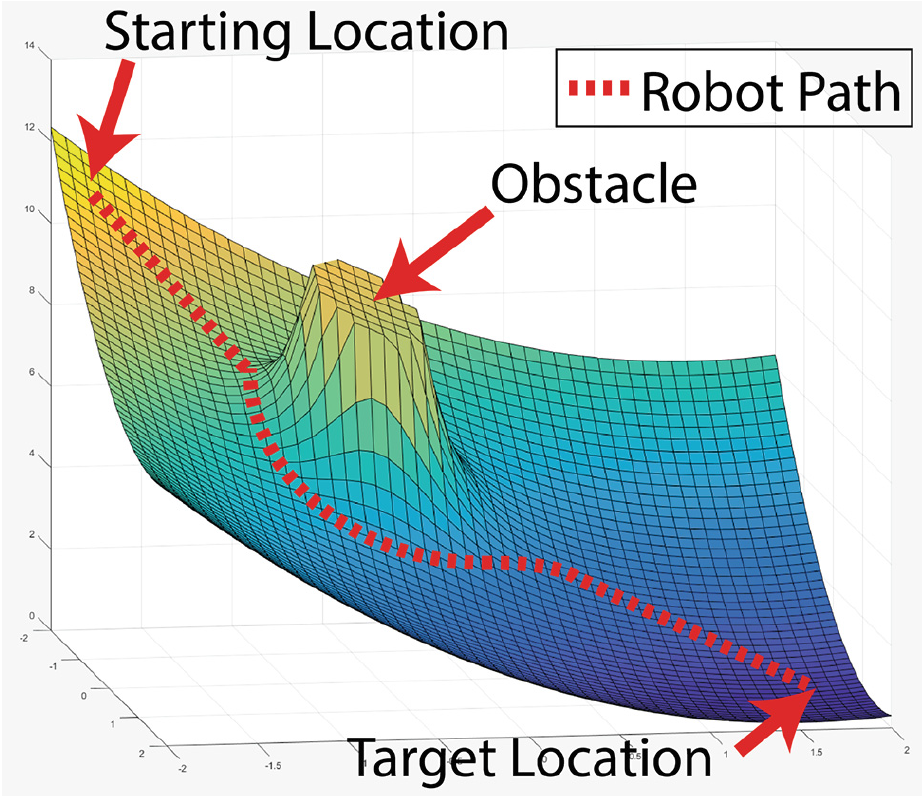
\includegraphics[scale=0.4]{potential_field}
	\caption{Example of artificial potential field}
	\label{potential_field}
\end{figure}
Given a point in the Cartesian space a virtual force is generated on that point by the potential field in the direction of the field gradient. 
\begin{equation}
\begin{split}
F^*_{target}&=-\nabla\mathcal{U}_{target}=-k\left(x-x_{goal}\right)^2 \\
F^*_{obstacle}&=-\nabla\mathcal{U}_{obstacle}=\begin{cases}\eta\left(\frac{1}{\rho}-\frac{1}{\rho_0}\right)\frac{1}{\rho^2}\frac{\partial\rho}{\partial x}& \text{if } \rho\leq\rho_0 \\
0 & \text{if } \rho>\rho_0
\end{cases}
\end{split}
\end{equation}
Multiple points can be chosen on the manipulator arm, to avoid collisions with all the links of the robot. The forces generated on all of these points are then projected on joint torques space through the Jacobian matrices. This way the manipulator arm, or the mobile robot, is induced by the joint torques to move away from the obstacles.\\
The system subjected to the artificial potential field is stable, but with approach it is very easy to run into local minima where the system is stable, but the robot is not in the target configuration.\\
With systems like Mobile Manipulators the obstacle avoidance problem can also be formulated as an optimization problem. Exploiting its increased number of joints a Mobile Manipulator can follow a primary task, i.e. trajectory traking of the end effector, while simoultaneously optimizing a secondary objective, and/or satisfying certain constraints by utilisation of the system's redundancy. In this sense, obstacle avoidance naturally arises as a secondary objective to be achieved, as explained in \cite{yamamoto2},\cite{tanner2000} or in \cite{perdereau2002}, where an obstacle avoidance term is added in the objective function of the optimization problem for the control of Mobile Manipulators
\begin{equation}
	\varphi_{OA}(q)=\sum_{i=1}^{l}\alpha_ip(\rho_i(q))
\end{equation}
Where $l$ is the number of points where the obstacle avoidance is considered, $\alpha$ is a weighting factor and $p$ is a penalty function depending on the distance of the point from the obstacle.\\
Another approach on Mobile Manipualators obstacle avoidance that deserves to be mentioned is the Elastic Strips method proposed in \cite{brockKhatib} where the motion of the robot is chosen between a set of homotopic collision-free paths through a potential field-based control algorithm. \\
A general issue that each approach has to deal with is the calculation of the minimum distance $\rho$ to an obstacle, and consequently the geometric modelling of the obstacles. More recent obstacle avoidance strategies (\cite{falconatale}) have overcome the complex 3D modelisation of the environment or of the robot. The approach is based on the exploitation of perception data available only from simple proximity sensors distributed on the robot, in order to deviate pre-planned motions exploiting the robot redundancy while executing the primary task. However, this strategy does not guarantee to complete the primary task in any environment.


